%% bare_jrnl_compsoc.tex
%% V1.4a
%% 2014/09/17
%% by Michael Shell
%% See:
%% http://www.michaelshell.org/
%% for current contact information.
%%
%% This is a skeleton file demonstrating the use of IEEEtran.cls
%% (requires IEEEtran.cls version 1.8a or later) with an IEEE
%% Computer Society journal paper.
%%
%% Support sites:
%% http://www.michaelshell.org/tex/ieeetran/
%% http://www.ctan.org/tex-archive/macros/latex/contrib/IEEEtran/
%% and
%% http://www.ieee.org/

%%*************************************************************************
%% Legal Notice:
%% This code is offered as-is without any warranty either expressed or
%% implied; without even the implied warranty of MERCHANTABILITY or
%% FITNESS FOR A PARTICULAR PURPOSE! 
%% User assumes all risk.
%% In no event shall IEEE or any contributor to this code be liable for
%% any damages or losses, including, but not limited to, incidental,
%% consequential, or any other damages, resulting from the use or misuse
%% of any information contained here.
%%
%% All comments are the opinions of their respective authors and are not
%% necessarily endorsed by the IEEE.
%%
%% This work is distributed under the LaTeX Project Public License (LPPL)
%% ( http://www.latex-project.org/ ) version 1.3, and may be freely used,
%% distributed and modified. A copy of the LPPL, version 1.3, is included
%% in the base LaTeX documentation of all distributions of LaTeX released
%% 2003/12/01 or later.
%% Retain all contribution notices and credits.
%% ** Modified files should be clearly indicated as such, including  **
%% ** renaming them and changing author support contact information. **
%%
%% File list of work: IEEEtran.cls, IEEEtran_HOWTO.pdf, bare_adv.tex,
%%                    bare_conf.tex, bare_jrnl.tex, bare_conf_compsoc.tex,
%%                    bare_jrnl_compsoc.tex, bare_jrnl_transmag.tex
%%*************************************************************************


% *** Authors should verify (and, if needed, correct) their LaTeX system  ***
% *** with the testflow diagnostic prior to trusting their LaTeX platform ***
% *** with production work. IEEE's font choices and paper sizes can       ***
% *** trigger bugs that do not appear when using other class files.       ***                          ***
% The testflow support page is at:
% http://www.michaelshell.org/tex/testflow/


\documentclass[10pt,conference,onecolumn,compsoc]{IEEEtran}


\usepackage{hyperref}
\usepackage{enumitem}
\setlist[itemize]{leftmargin=3 cm}
\setlist[enumerate]{leftmargin=3cm}



% *** CITATION PACKAGES ***
%
\ifCLASSOPTIONcompsoc
  % IEEE Computer Society needs nocompress option
  % requires cite.sty v4.0 or later (November 2003)
  \usepackage[nocompress]{cite}
\else
  % normal IEEE
  \usepackage{cite}
\fi
% cite.sty was written by Donald Arseneau
% V1.6 and later of IEEEtran pre-defines the format of the cite.sty package
% \cite{} output to follow that of IEEE. Loading the cite package will
% result in citation numbers being automatically sorted and properly
% "compressed/ranged". e.g., [1], [9], [2], [7], [5], [6] without using
% cite.sty will become [1], [2], [5]--[7], [9] using cite.sty. cite.sty's
% \cite will automatically add leading space, if needed. Use cite.sty's
% noadjust option (cite.sty V3.8 and later) if you want to turn this off
% such as if a citation ever needs to be enclosed in parenthesis.
% cite.sty is already installed on most LaTeX systems. Be sure and use
% version 5.0 (2009-03-20) and later if using hyperref.sty.
% The latest version can be obtained at:
% http://www.ctan.org/tex-archive/macros/latex/contrib/cite/
% The documentation is contained in the cite.sty file itself.



% *** GRAPHICS RELATED PACKAGES ***
%
\ifCLASSINFOpdf
   \usepackage[pdftex]{graphicx}
    \graphicspath{ {images/} }
 
\else
 
\fi
% graphicx was written by David Carlisle and Sebastian Rahtz. It is
% required if you want graphics, photos, etc. graphicx.sty is already
% installed on most LaTeX systems. The latest version and documentation
% can be obtained at: 
% http://www.ctan.org/tex-archive/macros/latex/required/graphics/
% Another good source of documentation is "Using Imported Graphics in
% LaTeX2e" by Keith Reckdahl which can be found at:
% http://www.ctan.org/tex-archive/info/epslatex/
%
% latex, and pdflatex in dvi mode, support graphics in encapsulated
% postscript (.eps) format. pdflatex in pdf mode supports graphics
% in .pdf, .jpeg, .png and .mps (metapost) formats. Users should ensure
% that all non-photo figures use a vector format (.eps, .pdf, .mps) and
% not a bitmapped formats (.jpeg, .png). IEEE frowns on bitmapped formats
% which can result in "jaggedy"/blurry rendering of lines and letters as
% well as large increases in file sizes.
%
% You can find documentation about the pdfTeX application at:
% http://www.tug.org/applications/pdftex









% *** PDF, URL AND HYPERLINK PACKAGES ***
%
\usepackage{url}
% url.sty was written by Donald Arseneau. It provides better support for
% handling and breaking URLs. url.sty is already installed on most LaTeX
% systems. The latest version and documentation can be obtained at:
% http://www.ctan.org/tex-archive/macros/latex/contrib/url/
% Basically, \url{my_url_here}.




\begin{document}

\title{GambleMania\\ for UTM CSCI 352}
%
%

% received ..."  text while in non-compsoc journals this is reversed. Sigh.

\author{Collin Winstead, Diego Arriaga% <-this % stops a space
}

\IEEEtitleabstractindextext{%
\begin{abstract}
This app allows the user to play three standard casino games: blackjack, three-card poker, and roulette. The player will play against an AI dealer in the blackjack and three-card poker games. In roulette, the program will randomly generate values from the roulette wheel. None of the games in our app will not require any real money to play; all money is virtual and has no monetary value. Users will have their own accounts which will contain login information and the account's balance. This information will be managed with a database.
\end{abstract}

}


% make the title area
\maketitle



\IEEEdisplaynontitleabstractindextext

\IEEEpeerreviewmaketitle



\section{Introduction}


Our project is called GambleMania. It will allow you to play the typical casino games of blackjack, three-card poker, and roulette. The player's balance will be saved in a database along with their login information. We decided to do this project because we thought it would be fun and require a good bit of research and work to finish. As for why we chose the games previously mentioned, it's because they are all fairly simple games to learn and play (probably by design). Because they are fairly simple, they should be relatively easy to program. Our target audience is adults 18 years old and older because the games featured in out app are all typically played in casinos. We expect our audience to use our app simply for fun or to practice blackjack or three-card poker. We did not include roulette in this list because roulette is based solely on randomness, so you can't really practice it.



\subsection{Background}
Minimally, we expect the user to know how to play blackjack, three-card poker, and roulette. However, we could implement a tutorial as a stretch goal to remove this requirement.

\subsection{Impacts}
Although our project is very small and limited, if distributed the project could possibly have a cultural impact by getting more people into the games of blackjack, three-card poker, and roulette. It could also potentially be used for data research and game theory by simulating thousands or millions of blackjack, three-card poker, and roulette games.

\subsection{Challenges}
We foresee the most challenging part of this project as the way the AI dealer will work in the blackjack and three-card poker games. These games have certain rules that need to be checked. For example, in the blackjack game, the dealer must stand on 17. In three-card poker, the player's hand must be checked against the dealer's hand. We think these kinds of obstacles will be our biggest hurdles.


\section{Scope}
This project will be completed when we have implemented a navigable main menu and the games of blackjack, three-card poker, and roulette. The main menu should minimally allow the user to navigate between games by clicking a button (one for each game) and return to desktop by clicking an exit button. The user must be able to play an accurate game of blackjack with the rules of dealer stands on 17 and blackjack pays 3:2. The user must be able to play an accurate game of three-card poker. A fully functioning roulette table must be implemented. Finally, each of the 56 individual cards in a standard deck of playing cards must be designed.


As mentioned earlier in this paper, there are a few stretch goals we can potentially meet should we be able to do so:\\

\begin{enumerate}
\item Create a tutorial for each game for users who do not know how to play.
\item Add more games to the app.
\item Make the main menu and game environments look better.
\item Create a Texas Hold'em style poker game that can be played over a network connection.
\end{enumerate}

\subsection{Requirements}
As mentioned in the Scope section, there are many basic requirements that need to be completed in order for this project to be done. There are also a few stretch goals that we could implement should we get done early. The basis of the basic requirements stems from the rules of play for each of the three basic games we will be implementing. There are also requirements that involve the UI design, some of which are simply required for a functional app and others are for a good-looking app. The non-functional requirements are based on how the user will interact with our app. These requirements are not necessarily required for the app to function, but are important for the users of our app.

\subsubsection{Functional}
\begin{itemize}
\item A button that exits the program in the main menu and in each of the games.
\item Buttons to navigate from the main menu to each of the games.
\item A back button in each game that navigates the user back to the main menu.
\item Game logic for each game.
\item A Microsoft Access database that stores user login information and user balances.
\end{itemize}

\subsubsection{Non-Functional}
\begin{itemize}
\item User login data and balance is hashed.
\item The app should be responsive and perform well without any major dips in framerate.
\item When the user's balance is modified, it should be updated in the database as soon as possible.
\item The app should be flexible enough so that it is possible to scale it up in the future.
\end{itemize}

\subsection{Use Cases}
This section defines and ranks the use cases for our project. A table of use cases is shown in Table \ref{tab:useCaseIndex}.

\begin{table}
\centering
\begin{tabular}{|c|c|c|c|c|c|}
\hline
Use Case ID & Use Case Name & Primary Actor & Complexity & Priority \\
\hline \hline
1 & Log In & User & Easy & 1\\
\hline
2 & Sign Up & User & Med & 1\\
\hline
3 & Play Blackjack & User & Easy & 3\\
\hline
4 & Play Three-Card Poker & User & Easy & 4\\
\hline
5 & Play Roulette & User & Hard & 5\\
\hline
6 & Watch a Tutorial & User & Easy & 6\\
\hline
7 & Navigate the Main Menu & User & Easy & 2\\
\hline
8 & Exit the Program & User & Easy & 1\\
\hline
\end{tabular}
\caption{Use Cases}
\label{tab:useCaseIndex}
\end{table}

\subsubsection{Use Case 1: Log In}
See Figure \ref{fig:login}
\begin{enumerate}
\item User enters their username and password into the provided text fields.
\item User clicks submit.
\item If the username and password are found in the database, the user proceeds to the main menu. Otherwise, the user must keep entering the username and password until the username and password matches.
\end{enumerate}

\subsubsection{Use Case 2: Sign Up}
See Figure \ref{fig:login}
\begin{enumerate}
\item User enters the username and password for their new account.
\item User clicks submit.
\item Account is registered to the database and the user proceeds to the main menu with the new account. The new account will have a starting balance of \$1000.
\end{enumerate}

\subsubsection{Use Case 3: Play Blackjack}
See Figure \ref{fig:blackjack}
\begin{enumerate}
\item User places an ante bet.
\item User and dealer are dealt two randomly chosen cards. 
\item User is shown a maximum of four options: Hit, Stand, Double Down, and Split. Double Down is only shown on the first turn. Split is only shown on the first turn when the user has two cards of the same face.
\item If the user chooses the Hit option, the user will be dealt another card.
\item If the user chooses the Stand option, the dealer will begin their turn.
\item If the user chooses the Double Down option, the user will place a bet with the same value as the ante bet and be dealt another card. After this, the dealer's turn begins.
\item If the user chooses the Split option, the user's two cards will be split into separate hands. Each hand will be dealt another card, giving the user two hands with two cards each. The user can play each hand separately.
\item After the user's turn is over, the dealer's turn begins. The dealer uses the same options the user has.
\item After the dealer's turn is over the user's hand and the dealer's hand are compared. The hand with the closest point value to 21 is the winner.
\item After the game is over, the user may enter another ante bet or exit to the main menu.
\end{enumerate}

\subsubsection{Use Case 4: Play Three-Card Poker}
See Figure \ref{fig:three-card}
\begin{enumerate}
\item User places an ante bet and optionally a pair plus bet.
\item User and dealer are dealt three cards.
\item User is shown two options: Play and Fold.
\item If the user chooses the Play option, the user will make a bet that has the same value as the ante bet. After this, the user's turn will be over.
\item If the user chooses the Fold option, the user will cede their hand to the dealer and lose automatically.
\item After the user's turn is over, the dealer's turn begins. The dealer will reveal their cards and compare its hand with the user's.
\item If the dealer's hand is not better than Queen high or the user's hand is better, the user wins. Otherwise, if the dealer has the better hand, the dealer wins.
\item After the game is over, the user may enter another ante bet/pair plus bet or exit to the main menu.
\end{enumerate}

\subsubsection{Use Case 5: Play Roulette}
See Figure \ref{fig:roulette}
\begin{enumerate}
\item User places a bet of their choice on any valid space on the board.
\item Once the user is done betting, the user may click the ``Spin" button to spin the wheel.
\item Once the ball in the roulette wheel rests in a slot, that slot determines what values win.
\item The user is paid out according to what bet they made and where the ball landed.
\item The user may choose to place another bet or exit to the main menu once the payout - or lack thereof - is done.
\end{enumerate}

\subsubsection{Use Case 6: Watch a Tutorial}

\begin{enumerate}
\item In the main menu, the user may click the button labeled ``Watch a Tutorial."
\item Once in the tutorial screen, the user may select any of the tutorials associated with the three games in the app.
\item Once the user clicks on a tutorial, they will be shown a video that teaches the user how to play the game.
\item Once the user is done watching the tutorial, they may go back to the tutorials screen.
\item From the tutorials screen, the user may choose to watch another tutorial or exit to the main menu.
\end{enumerate}

\subsubsection{Use Case 7: Navigate the Main Menu}
See Figure \ref{fig:main}
\begin{enumerate}
\item The user can click the ``Blackjack" button to go to the blackjack game screen.
\item The user can click the ``Three-Card Poker" button to go to the three-card poker game screen.
\item The user can click the ``Roulette" button to go to the roulette game screen.
\item The user can click the ``Log Out" button to log out of their account and go back to the log in/sign up screen.
\item The user can click the ``X" button at the top right corner of the screen to exit the program.
\end{enumerate}

\subsubsection{Use Case 8: Exit the Program}
See Figure \ref{fig:main}
\begin{enumerate}
\item The user can click the ``X" button at the top right corner of the main menu screen to exit the program.
\end{enumerate}

\newpage
\subsection{Interface Mockups}

\begin{figure}[h]
\caption{Login/sign-up GUI mockup}
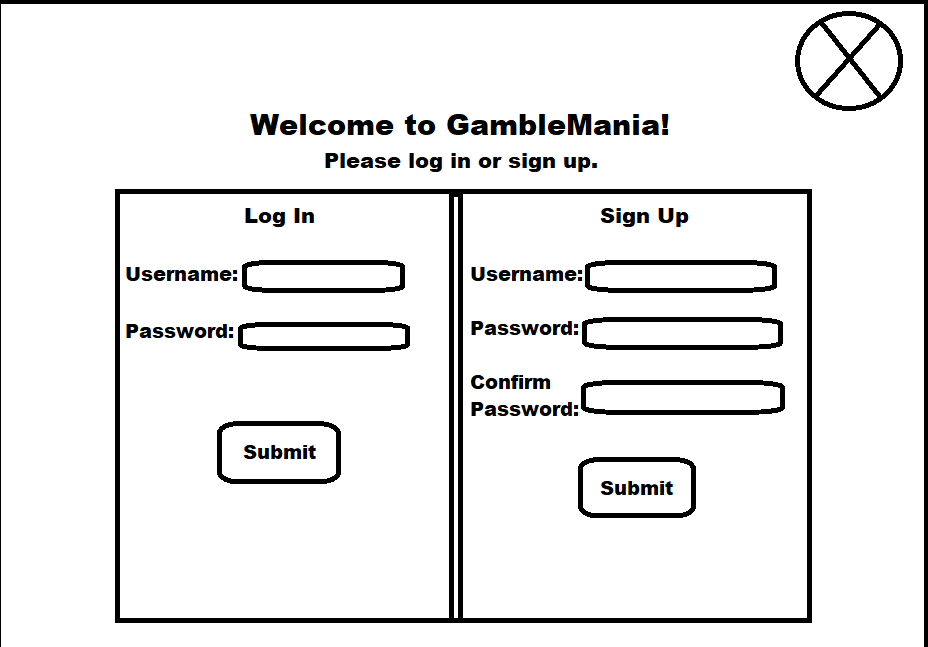
\includegraphics[scale=0.4]{login}
\label{fig:login}
\centering
\end{figure}

\begin{figure}[h]
\caption{Main menu GUI mockup}
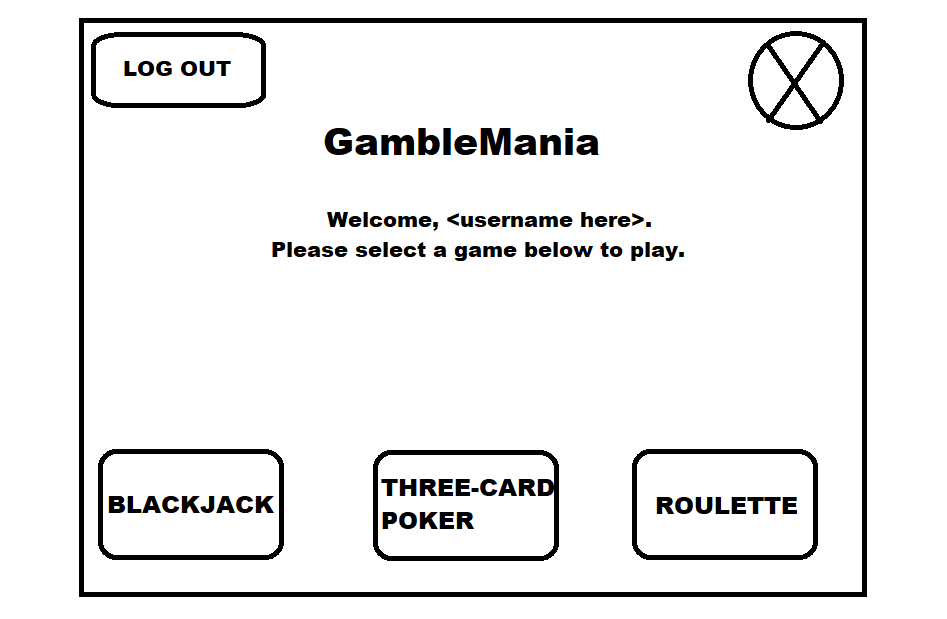
\includegraphics[scale=0.4]{main}
\label{fig:main}
\centering
\end{figure}

\newpage

\begin{figure}[h]
\caption{Blackjack GUI mockup}
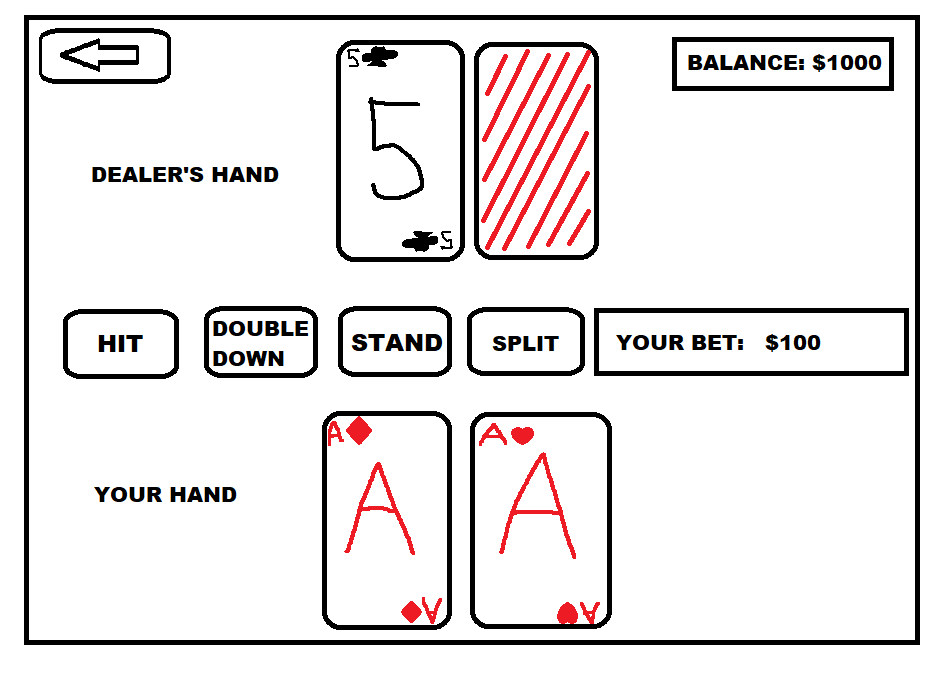
\includegraphics[scale=0.4]{blackjack}
\label{fig:blackjack}
\centering
\end{figure}

\newpage

\begin{figure}[h]
\caption{Three-card poker GUI mockup}
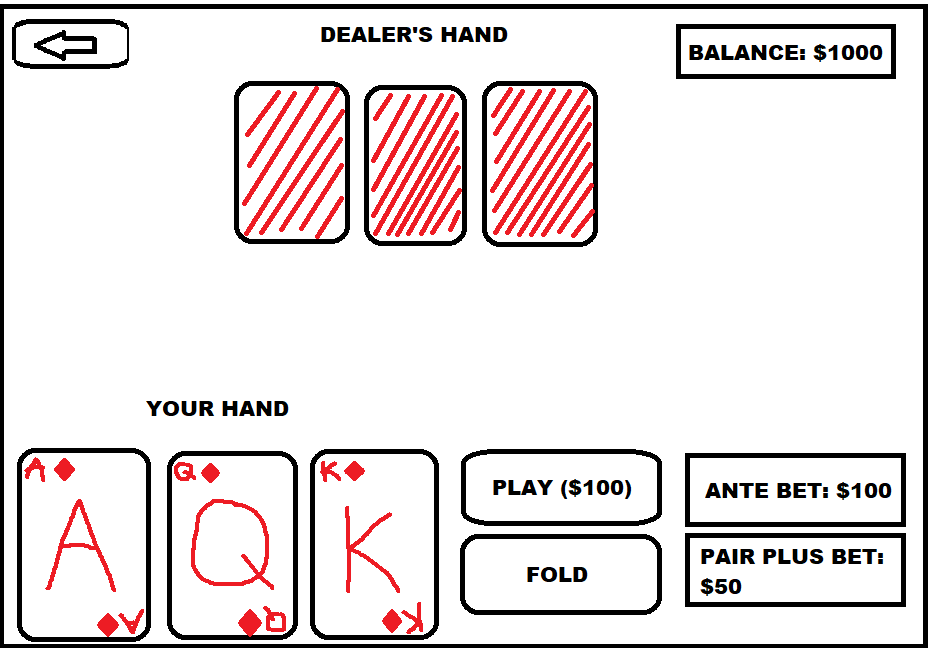
\includegraphics[scale=0.4]{three-card}
\label{fig:three-card}
\centering
\end{figure}

\begin{figure}[h]
\caption{Roulette GUI mockup}
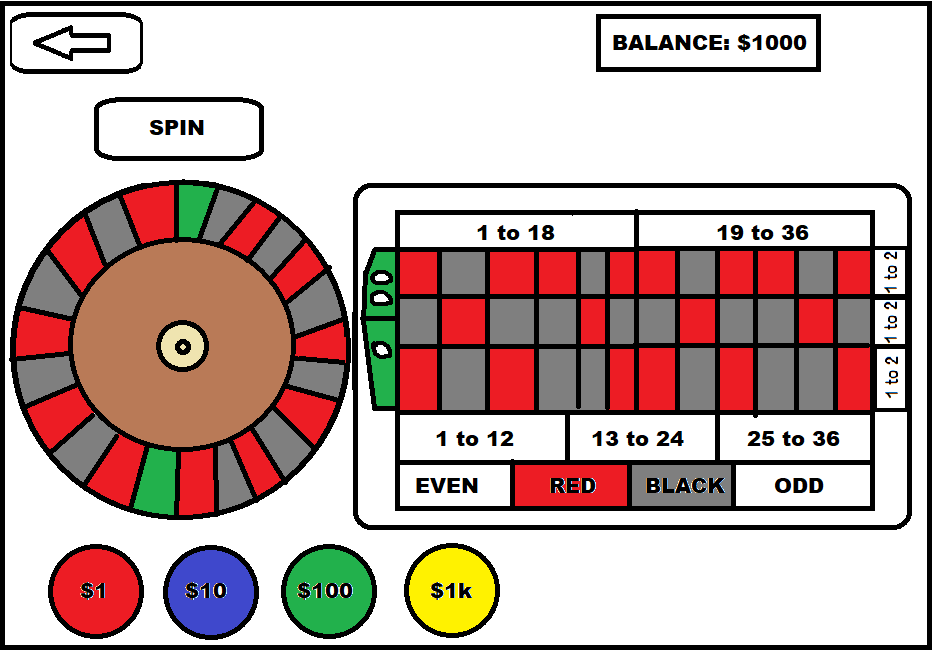
\includegraphics[scale=0.4]{roulette}
\label{fig:roulette}
\centering
\end{figure}

\newpage

\section{Timeline}
This section describes the timeline of our project.\\
\newline
8/27 - Finding partners.\\
9/2 - Formed a team.\\
9/9 - Created a rough draft of the project proposal.\\
9/16 - Designed a plan of action for the project.\\
9/23 - Worked on the GUI mockups and the Requirements and Use Cases sections of the project proposal.\\
9/30 - Updated the GUI mockups.\\
10/7 - Researched potential design patterns for the project.\\
10/14 - Modified the Use Cases section of the project proposal.\\
10/21 - Midterms\\
10/28 - Added the Timeline and Project Structure \& UML Outline sections. Begin implementing the login/sign-up screen and database.\\
11/4 - Begin work on blackjack and three-card poker. Login/sign-up should be done by this point.\\
11/11 - We should be about halfway done with blackjack and three-card poker by this point.\\
11/18 - Begin work on roulette. Blackjack and three-card poker should be done by this point.\\
11/25 - Begin work on the presentation and work on stretch goals such as the tutorials.\\
12/2 - Demo the project. The project should be finished by this point.\\

\section{Project Structure \& UML Outline}

\begin{figure}[h]
\caption{UML Outline}
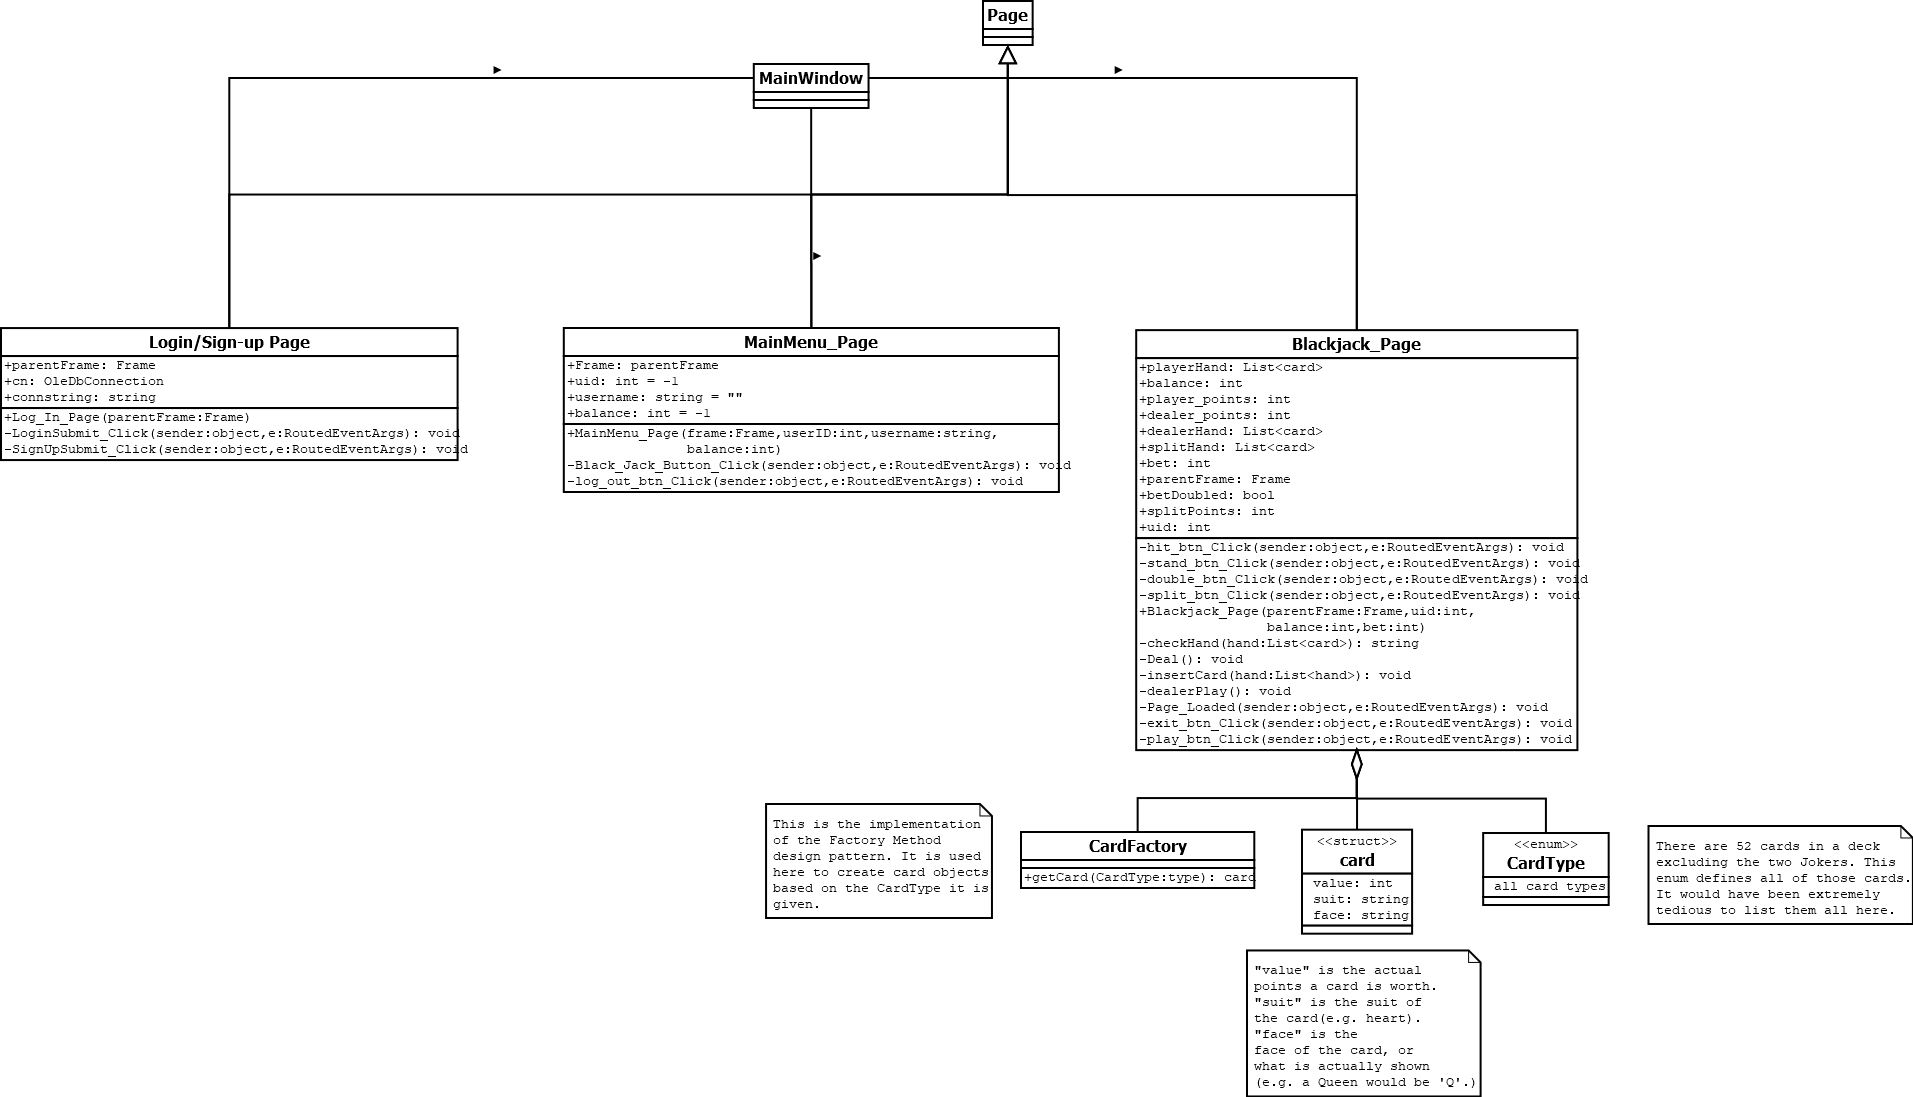
\includegraphics[scale=0.4]{GameDesign}
\label{fig:outline}
\centering
\end{figure}

\noindent
This section covers the overall project structure and provides a UML outline of the project (see Figure \ref{fig:outline}).\\
\newline
The project's structure hinges on a NavigationWindow object. A NavigationWindow allows easy navigation between pages in a WPF app. Initially, our project will contain five pages, but more could be added depending on how much time we have left by December 2. The initial five pages are named Login/Sign-Up, Roulette, Main Menu, Blackjack, and Three-Card Poker. Each page will contain Label and Button objects. The game pages will also contain their respective game classes.\\
\newline
Each game class contains the GetBalance and UpdateBalance methods and depends on a card struct. As the names imply, these methods get and modify the user's balance in the database. The card struct defines the three attributes of a card: value, suit, and display (or face). Roulette has its own unique game class called RouletteGame. This class has two unique methods: Spin and PlaceBet. The Spin method will play an animation of the roulette wheel spinning and determine whether the user wins or loses. PlaceBet determines what bet the user made for which slot on the board and calls UpdateBalance accordingly.\\
\newline
The Blackjack page contains the BlackjackGame class, which inherits from an abstract CardGame class like the Three-Card class. The CardGame class contains two unique methods: Deal and ChangeWinState. Deal simply deals out cards to the player and dealer. ChangeWinState updates the win state depending on if the player wins or loses. The BlackjackGame class has several unique methods: Hit, Stand, DoubleDown, Split, Bust, and Blackjack. Hit, Stand, DoubleDown, and Split are all actions that the user can take on their turn. Bust is called if either the player or dealer has a point value of over 21. Blackjack is called if either the player or dealer has a point value of 21 on the first turn.\\
\newline
Finally, the Three-Card class also has several unique methods: AnteBet, PairPlusBet, Fold, PlayHand, DealerRevealHand, and CompareHands. AnteBet, PairPlusBet, Fold, and PlayHand are all actions that the user can take on their turn. DealerRevealHand is called after the user is finished with their turn, and reveals the dealer's hand to the user. CompareHands is called after the dealer reveals their hand, and determines which hand is better: the user's or the dealer's.

% that's all folks
\end{document}
